\section{VL vom 25.~November 2010}
$\beta[x/a]$ (ersetze das x durch a.
\seeslide{37}

\subsection{Beispiel FO-Auswertung}

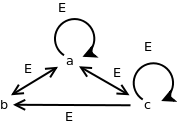
\includegraphics[width=4cm]{25_11_10_1.png}

\begin{itemize}
  \item $\varphi = \forall x.(x=z \OR \forall y.E(x,y))$
  \item $\beta(z) = b$
\end{itemize}

\begin{verbatim}
  Rekursionsbaum von Bernd tikzen
\end{verbatim}

\subsubsection{Auswertung Korrektheit/Platzbedarf}

\begin{enumerate}
  \item Einfach per Induktion über die Struktur von $\phi$ (die Fälle
  des Algorithmus spiegeln Semantik der Operatoren wieder).
  
  \item Die elementaren Berechnungsschritte können offensichtlich mit
  polynomiell viel Platz ausgeführt werden. Ansonsten muss nur in den
  Fällen $\exists x.\psi$ und $\forall x.\psi$ das aktuelle $a$
  gespeichert werden. Da die Rekursionstiefe offensichtlich durch
  $st(\psi)$ begrenzt ist, benötigt auch der Rekursionsstack nur
  polynomiell viel Platz.
\end{enumerate}

\subsection{FO und Datenbanken}

\begin{align*}
  \text{Film}^{\Afrak} &= \set{
                                  (\text{Die Vögel}, 1963, \text{Hitchcock}),
                                  (\text{Marnie}, 1964, \text{Hitchcock}),
                                  \dots
                                } \\
  \text{Schauspieler}^{\Afrak} &= \set{(\text{Connery}, \text{Marnie}), \dots}
\end{align*}

\subsection{Beispiel Domänenunabhängigkeit}
\seeslide{41}
Beispiele für domänenabhängige FO-Formeln

\begin{tabular}{@{}*{2}{>{$}l<{\quad$}@{}}}
  \varphi = \NOT P(x) & \\
  \Afrak:_{P(a)}                     & \Afrak':_{P(a) \qquad a'} \\
  \ans(\Afrak, \varphi) = \emptyset  & \ans(\Afrak', \varphi) = \set{a'} \\
  \varphi' = P(x) \OR \exists y.P(y)       & \\
  \ans(\Afrak, \varphi') = \set{a}   & \ans(\Afrak', \varphi') = \set{a, a'} \\
\end{tabular}

Alle Übersetzungen von Kern-SQL-Anfragen in FO sind domänenunabhängig, z.B.
\[
  \exists y. \text{Film}(\underline{x}, y, \text{Hitchcock})
\]

Funktionale Vollständigkeit. Es reichen $\NOT,\AND$ und $\exists$\\
\seeslide{46,47}

\subsection{Erfüllbarkeit, Gültigkeit, Kosequenz}

Beispiele

Die folgenden Formeln sind gültig
\begin{itemize}
  \item $\forall x.\exists y. y=f(x)$
  \item $f(x) = x \IMPL f(f(x)) = x$
\end{itemize}

Die folgende Formeln ist erfüllbar, aber nur in unendlich großen Modellen:
\begin{itemize}
  \item $\forall x.\exists y. P(x,y)
  \AND \forall x,yz. P(x,y) \AND P(y,z) \IMPL P(x,z)
  \AND \NOT\exists x. P(x,x)$
  \item transitiv, keine reflexive P-Schleife
\end{itemize}

Konsequenz:
\begin{itemize}
  \item $\exists x.\forall y.(x=y) \models f(c)=c$
\end{itemize}


\subsection{Pränex-Normalform (PNN)}
\seeslide{52}

PNF, exemplarisch die erste Äquivalenz:

\begin{align}
  \Afrak, \beta &\models \varphi \OR \exists x.\psi \\
  \text{gdw.}\quad \Afrak, \beta &\models \varphi\ \text{oder es gibt}\ a\in A\ \text{mit}\ \Afrak, \beta[x/a] \models \psi \\
  \text{gdw. es gibt $a\in A$, so dass}\ \Afrak, \beta[x/a] &\models \varphi\ \text{oder}\ \Afrak, \beta[x/a] \models \psi\\
      & \qquad\qquad\text{(weil $x$ nicht frei in $\varphi$ vorkommt)} \\
  \text{gdw.}\quad \Afrak, \beta[x/a] &\models \exists x.(\varphi \OR \psi)
\end{align}

Beweis per Induktion über die Struktur von $\varphi$.
\begin{itemize}
  \item \textbf{IA}
  \begin{enumerate}
    \item Wenn $\varphi$ quantorenfrei ist, ist es schon in PNF.
    \item Sei $\varphi = \NOT\psi$. Nach IV gibt es PNF-Formel $\psi' = Q_1x_1\cdots Q_nx_n \vartheta$ mit $\psi' \EQUIV \psi$. Die Dualität von $\exists$ und $\forall$ liefert
      $\varphi = \overline{Q}_1x_1 \cdots \overline{Q}_nx_n.\NOT\vartheta$ (PNF)
    wobei $\overline{\exists}=\forall$ und $\overline{\forall}=\exists$.
    
    \item Sei $\varphi = \psi_1 \circ \psi_2$ mit $\circ\in\set{\AND,\OR}$
    Nach IV gibt es PNF-Formeln $\psi_1', \psi_2'$ mit $\psi_1 \EQUIV \psi_1'$
    und $\psi_2 \EQUIV \psi_2'$. Durch Variablenumbenennung erreichen wir, dass in
    
    \begin{align}
      \psi_1' &= Q_1x_1 \cdots Q_nx_n. \vartheta_1 \\
      \psi_2' &= Q_1'y_1 \cdots Q_m'y_m. \vartheta_2 \\
    \end{align}
    
    die $x_1,\dots,x_n, y_1,\dots,y_m$ paarweise verschieden und verschieden von allen freien Variablen in $\psi_1'$ und $\psi_2'$ sind.
    
    Offenbar ist
    
    \begin{align}
      \varphi' = Q_1x_1\cdots Q_nx_n Q_1'y_1 \cdots Q_m'y_m .(\vartheta\circ\vartheta)
    \end{align}
    
    in PNF. Da $y_1,\dots,y_m$ nicht in $\psi_1'$ vorkommen und $x_1,\dots,x_n$ nicht in $\psi_2'$, liefern die Äquivalenzen $\varphi \EQUIV \varphi'$
    
    \item Sei $\varphi = Q x.\psi$ mit $Q \in\set{\exists, \forall}$.
    IV liefert PNF-Formel $\psi'=Q_1x_1\cdots Q_nx_n.\vartheta$
    mit $\psi \EQUIV \psi'$. Durch Umbenennen, kann erreicht werden,
    dass $x \in \set{x_1,\dots,x_n}$. Dann ist $Q x.\psi'$ äquivalent zu $\varphi$ und in PNF.
  \end{enumerate}
\end{itemize}
\qed



